\chapter{Fragmentierungsdiagramme und MS-Spektren der MS-Leafspray Experimente}

Im Folgenden befinden sich Fragmentierungsdiagramme von Verbindungen, die mit MS-Leafspray erstellt wurden, aus diversen Gründen jedoch nicht im Hauptteil der Arbeit behandelt werden. Sie werden hier aufgelistet, um einen tieferen Einblick in die Fragmentierungsdiagramme zu bekommen und diese anhand des hiermit erhaltenen größeren Datensatzes selbst besser bewerten zu können. Auf eine eingehendere Erklärung und Analyse wird verzichtet.

\section{Reaktionsprodukt von Bo-DYCC}

\begin{figure}[!htbp]
  \begin{subfigure}[b]{0.5\textwidth}
    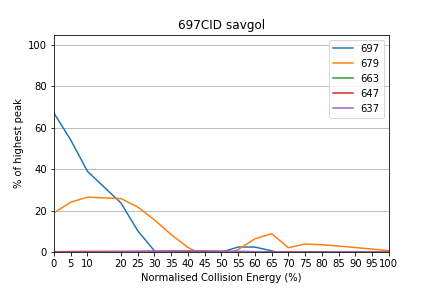
\includegraphics[width=\textwidth]{content/Anhang/MSLeafspray/RP_Bo-DYCC/697CID-697savgol.png}
    \caption{}
  \end{subfigure}
  \hfill
  \begin{subfigure}[b]{0.5\textwidth}
    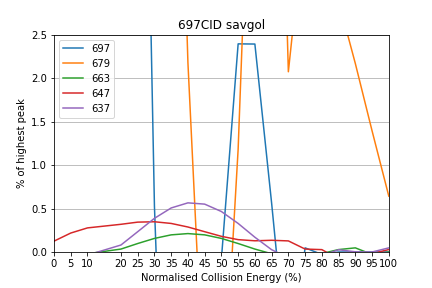
\includegraphics[width=\textwidth]{content/Anhang/MSLeafspray/RP_Bo-DYCC/697CID-697savgolv25.png}
    \caption{}
  \end{subfigure}
  
  \caption[Fragmentierungsdiagramme des Reaktionsproduktes von Bo-DYCC, Quelle: Autor]{Fragmentierungsdiagramme des Reaktionsproduktes von Bo-DYCC: (a) m/z = 697 [M+K]\textsuperscript{+} - es handelt sich dabei um das Anhydrid, (b) Ausschnitt aus (a)}
\end{figure}

\pagebreak
\section{Reaktionsprodukt von Bo-DNCC}

\begin{figure}[!htbp]
  \begin{subfigure}[b]{0.5\textwidth}
    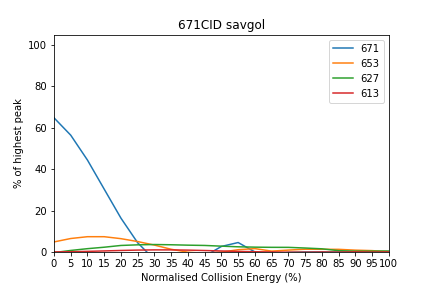
\includegraphics[width=\textwidth]{content/Anhang/MSLeafspray/RP_Bo-DNCC/671CID-671savgol.png}
    \caption{}
  \end{subfigure}
  \hfill
  \begin{subfigure}[b]{0.5\textwidth}
    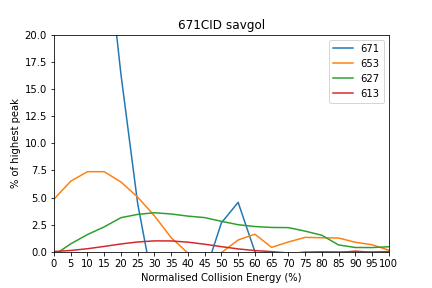
\includegraphics[width=\textwidth]{content/Anhang/MSLeafspray/RP_Bo-DNCC/671CID-671savgolv20.png}
    \caption{}
  \end{subfigure}
  
  \begin{subfigure}[b]{\textwidth}
    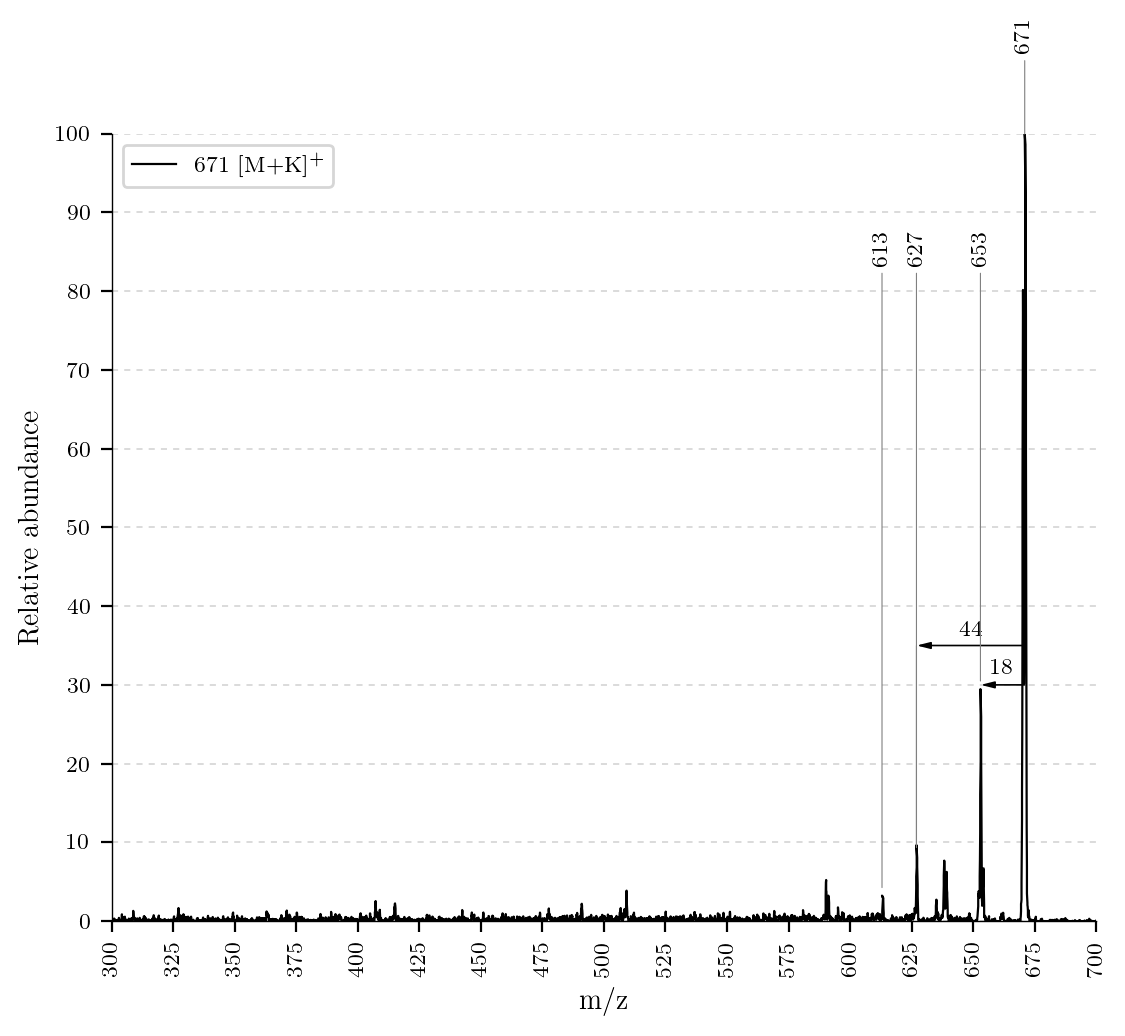
\includegraphics[width=\textwidth, height=0.5\textheight]{content/Anhang/MSLeafspray/RP_Bo-DNCC/VWA_MS_LeafSpray_671.png}
    \caption{}
  \end{subfigure}
  
  \caption[Fragmentierungsdiagramme und MS-Spektrum des Reaktionsproduktes von Bo-DNCC, Quelle: Autor]{Fragmentierungsdiagramme und MS-Spektrum des Reaktionsproduktes von Bo-DNCC: (a) m/z = 671 [M+K]\textsuperscript{+} - es handelt sich dabei um einen Methylester, (b) Ausschnitt aus Diagramm (a), (c) MS-Spektrum bei m/z = 671 [M+K]\textsuperscript{+}}
\end{figure}

\pagebreak
\section{Reaktionsprodukt von Chl-Katabolit mit m/z = 667 Da [M+K]\textsuperscript{+}}

\begin{figure}[!htbp]
  \begin{subfigure}[b]{0.5\textwidth}
    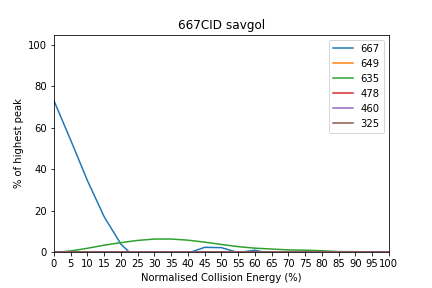
\includegraphics[width=\textwidth]{content/Anhang/MSLeafspray/RP_667/667CID-667savgol.png}
    \caption{}
  \end{subfigure}
  \hfill
  \begin{subfigure}[b]{0.5\textwidth}
    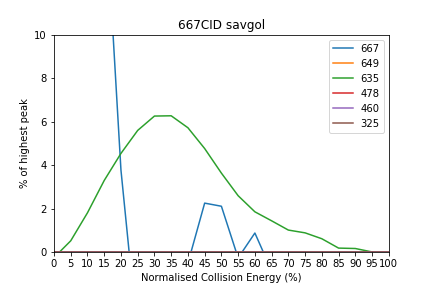
\includegraphics[width=\textwidth]{content/Anhang/MSLeafspray/RP_667/667CID-667savgolv10.png}
    \caption{}
  \end{subfigure}
  
  \begin{subfigure}[b]{\textwidth}
    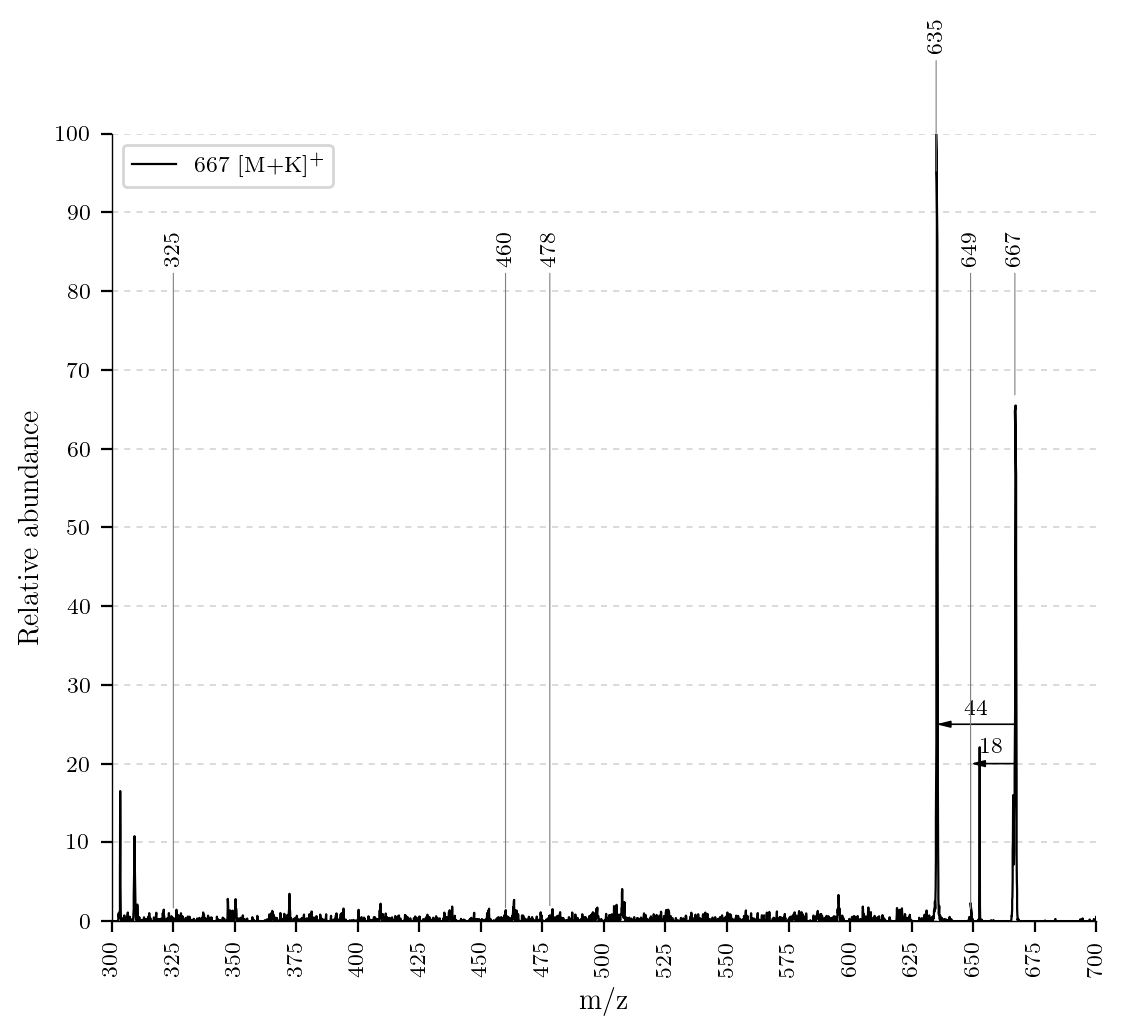
\includegraphics[width=\textwidth, height=0.5\textheight]{content/Anhang/MSLeafspray/RP_667/VWA_MS_LeafSpray_667.png}
    \caption{}
  \end{subfigure}
  
  \caption[Fragmentierungsdiagramme und MS-Spektrum eines vermeintlichen Chl-Kataboliten mit m/z = 667 Da, Quelle: Autor]{Fragmentierungsdiagramme und MS-Spektrum eines vermeintlichen Chl-Kataboliten mit m/z = 667 [M+K]\textsuperscript{+}: (a) Fragmentierungsdiagramm, (b) Ausschnitt aus Diagramm (a), (c) MS-Spektrum bei m/z = 667 [M+K]\textsuperscript{+}}
\end{figure}